\chapter{Datasets and Evaluation Methodology}
\label{ch:methodology}

This chapter sets out the experimental foundation shared by the three
perception sub-tasks studied in the thesis. Because the ball, court, and bounce
comparisons each reuse the same datasets, split contracts, and metric
definitions, these elements are described once here rather than repeated in
every results chapter. Section~\ref{sec:meth-tracknet} describes the TrackNet
tennis dataset, which underlies both ball tracking and bounce detection, and
Section~\ref{sec:meth-court} describes the separate court-keypoint dataset used
for court detection. Section~\ref{sec:meth-noncompare} states explicitly that
the two datasets are not cross-comparable. Section~\ref{sec:meth-splits} defines
the deterministic split policies, and Section~\ref{sec:meth-metrics} defines the
shared metric vocabulary. Task-specific preprocessing, learning targets, and
training details are not covered here: they belong with the models that consume
them and are presented in Chapters~\ref{ch:ball}, \ref{ch:court},
and~\ref{ch:bounce} respectively.

\section{The TrackNet Tennis Dataset}
\label{sec:meth-tracknet}

Ball tracking and bounce detection are both evaluated on the publicly available
tennis dataset released with the original TrackNet work
\cite{huang2019tracknet}. The dataset is drawn from broadcast tennis video and
is organised into ten matches, named game1 through game10.
Each match is divided into short clips of consecutive frames, with one clip per
folder containing the extracted JPEG frames and a single annotation file,
Label.csv. In the copy used in this work the dataset comprises 95 clips
and 19{,}835 annotated frames in total; its composition per match is given in
Table~\ref{tab:tracknet-games}.

\begin{table}[h]
  \centering
  \caption{Composition of the TrackNet tennis dataset by match, as used in this
    thesis. Both the ball-tracking and bounce-detection comparisons draw from
    this same pool of frames.}
  \label{tab:tracknet-games}
  \begin{tabular}{lrr}
    \toprule
    Match & Clips & Frames \\
    \midrule
    game1  & 13 & 1{,}978 \\
    game2  &  8 & 2{,}222 \\
    game3  &  9 & 1{,}888 \\
    game4  &  7 & 2{,}238 \\
    game5  & 15 & 1{,}964 \\
    game6  &  4 & 1{,}989 \\
    game7  &  9 & 1{,}881 \\
    game8  &  9 & 1{,}958 \\
    game9  &  9 & 1{,}573 \\
    game10 & 12 & 2{,}144 \\
    \midrule
    Total & 95 & 19{,}835 \\
    \bottomrule
  \end{tabular}
\end{table}

\subsection{Annotation schema}
\label{sec:meth-tracknet-schema}

Every row of a ``Label.csv'' file annotates one frame with five fields:
the frame file name, a visibility class, the ball x-coordinate and
y-coordinate in image pixels, and a status label. The visibility
field follows the dataset's four-level convention: class~0 marks frames in which
the ball is outside the frame or otherwise not visible; class~1 marks frames in
which the ball is easily identifiable; class~2 marks frames in which the ball is
present but difficult to identify, for example under motion blur; and class~3
marks frames in which the ball is occluded by another object. The status field
records, independently of visibility, whether a salient event occurs at that
frame: status~0 denotes ordinary in-flight frames with no event, status~1 a
racket hit, and status~2 a ball bounce on the court. Because a hit or a bounce
is defined by how the ball moves rather than by its appearance in a single
frame, Figure~\ref{fig:status-classes} illustrates each status value with the
ball trajectory over a short window around an example event, while
Figure~\ref{fig:visibility-classes} illustrates each visibility class with a
representative frame and a magnified view of the ball region. The distribution
of both labels across the full dataset is summarised in
Table~\ref{tab:tracknet-labels}. The ball is clearly visible in roughly 89\% of
frames, while bounce events, the target of Chapter~\ref{ch:bounce}, account for
only about 2.6\% of frames, a sparsity that directly shapes the choice of
evaluation metric for that task (Section~\ref{sec:meth-metrics-event}).

\begin{table}[h]
  \centering
  \caption{Label distribution across all 19{,}835 frames of the TrackNet
    dataset. Visibility and status are annotated independently of one another.}
  \label{tab:tracknet-labels}
  \begin{tabular}{llrr}
    \toprule
    Field & Class & Frames & Share \\
    \midrule
    Visibility & 0: not visible        &    729 &  3.7\% \\
               & 1: easily visible     & 17{,}632 & 88.9\% \\
               & 2: hard to identify   &  1{,}392 &  7.0\% \\
               & 3: occluded           &     82 &  0.4\% \\
    \midrule
    Status     & 0: in flight (none)   & 18{,}796 & 94.8\% \\
               & 1: hit                &    516 &  2.6\% \\
               & 2: bounce             &    523 &  2.6\% \\
    \bottomrule
  \end{tabular}
\end{table}

\begin{figure}[t]
  \centering
  \begin{subfigure}{0.49\textwidth}
    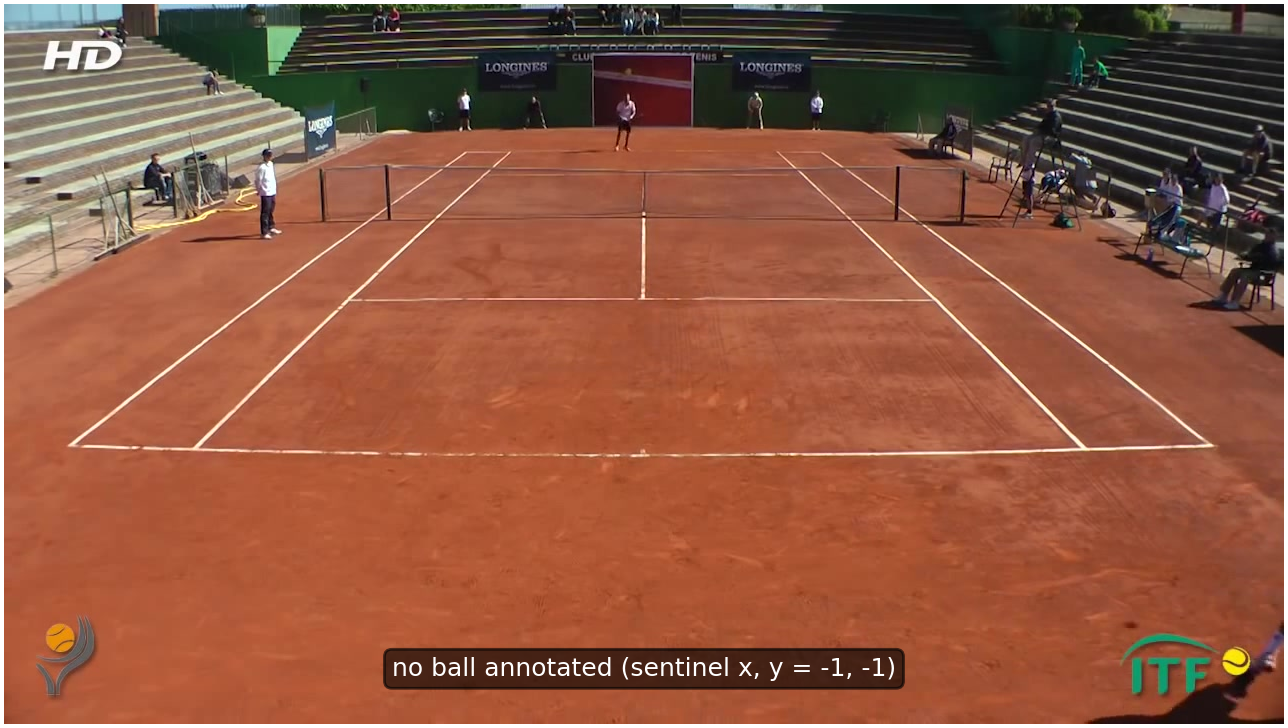
\includegraphics[width=\linewidth]{img/visibility_class0.png}
    \caption{Class 0: ball not visible}
  \end{subfigure}\hfill
  \begin{subfigure}{0.49\textwidth}
    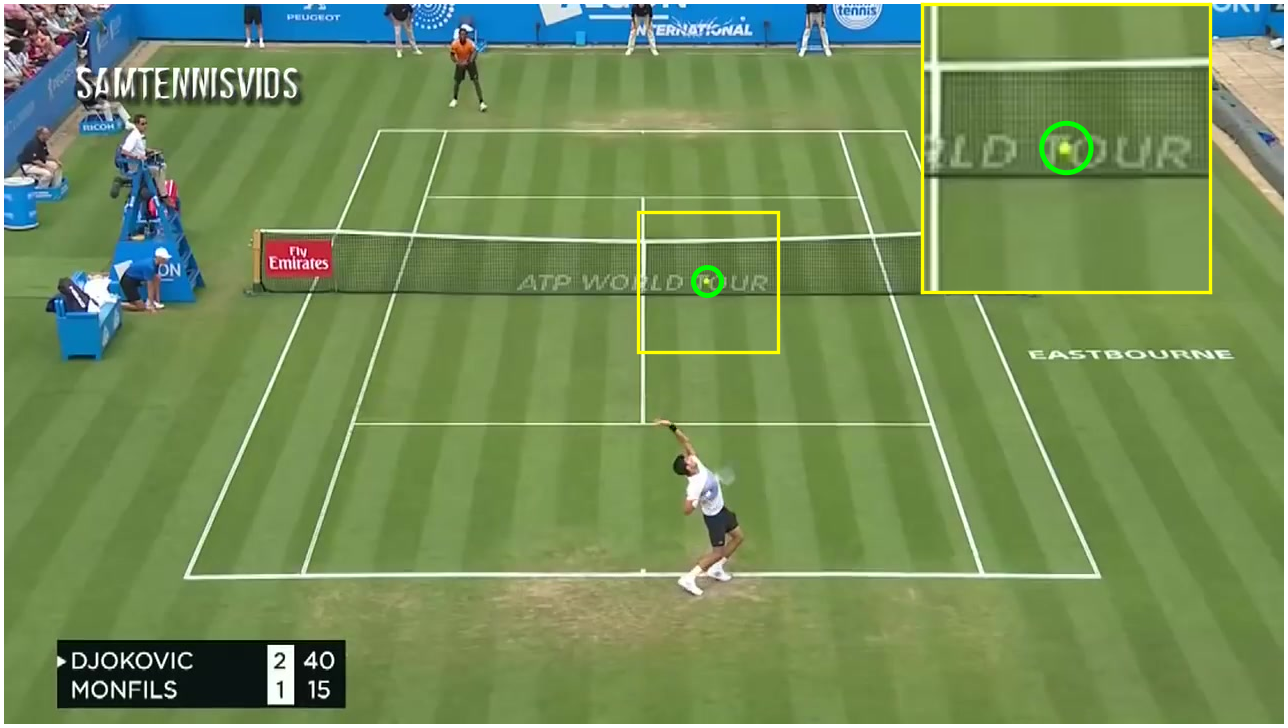
\includegraphics[width=\linewidth]{img/visibility_class1.png}
    \caption{Class 1: easily visible}
  \end{subfigure}

  \vspace{0.6em}
  \begin{subfigure}{0.49\textwidth}
    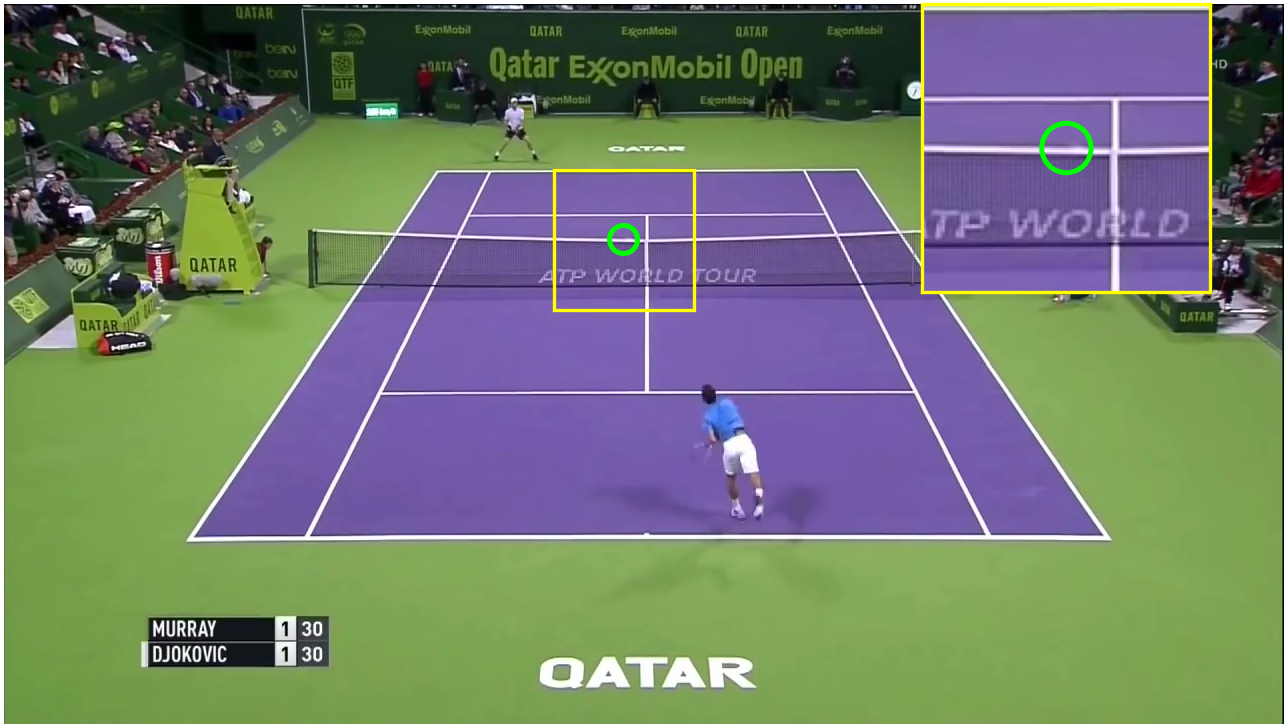
\includegraphics[width=\linewidth]{img/visibility_class2.png}
    \caption{Class 2: hard to identify}
  \end{subfigure}\hfill
  \begin{subfigure}{0.49\textwidth}
    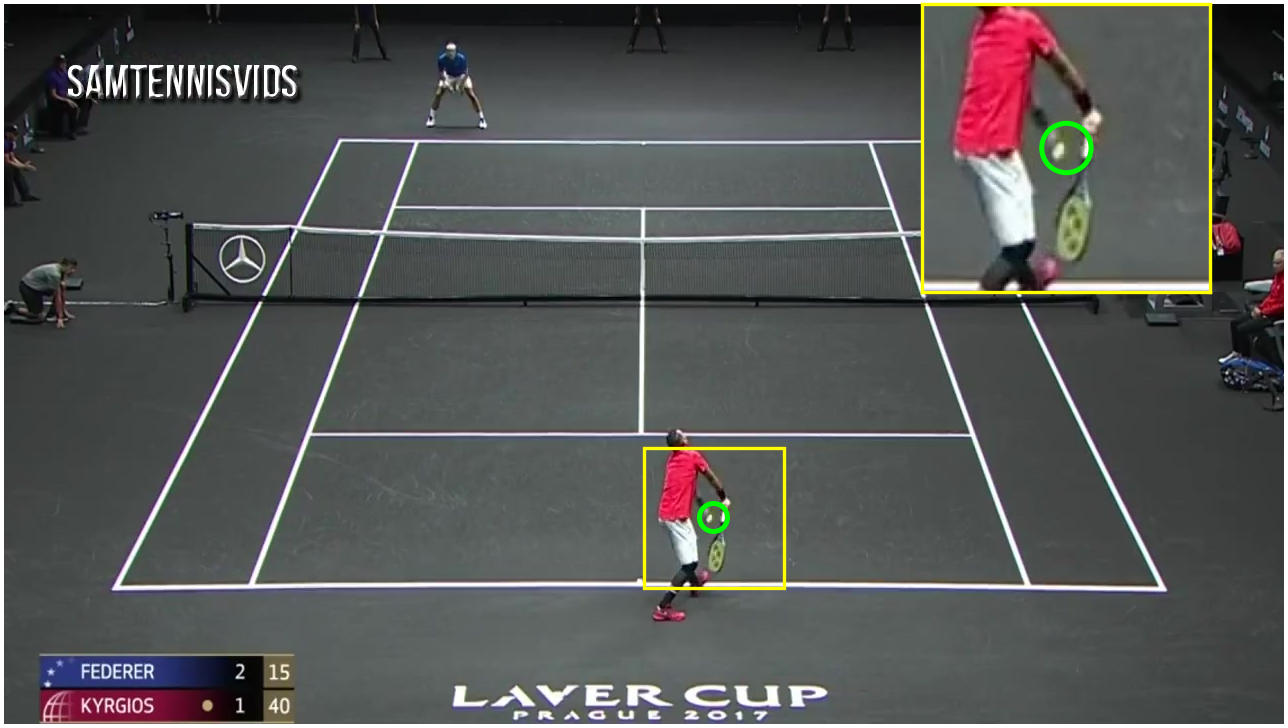
\includegraphics[width=\linewidth]{img/visibility_class3.png}
    \caption{Class 3: occluded}
  \end{subfigure}
  \caption{Representative frames for the four TrackNet visibility classes. In
    each panel the ground-truth ball position is marked with a green circle and
    magnified in the yellow inset; class~0 carries no ball annotation. The
    examples are drawn from different matches and court surfaces (clay, grass,
    and hard court), which also illustrates the visual variety of the dataset.}
  \label{fig:visibility-classes}
\end{figure}

Throughout the pipeline, a single encoding of the absence of a ball is used: when an
annotation carries visibility~0, or its coordinate fields are blank or negative,
the ball position is represented as $(-1, -1)$. This convention is preserved by
every dataset loader, model output, and metric in both the ball and bounce
projects, so that ``no ball'' is always distinguishable from a coordinate that
happens to lie near the image origin.

\begin{figure}[t]
  \centering
  \begin{subfigure}{0.32\textwidth}
    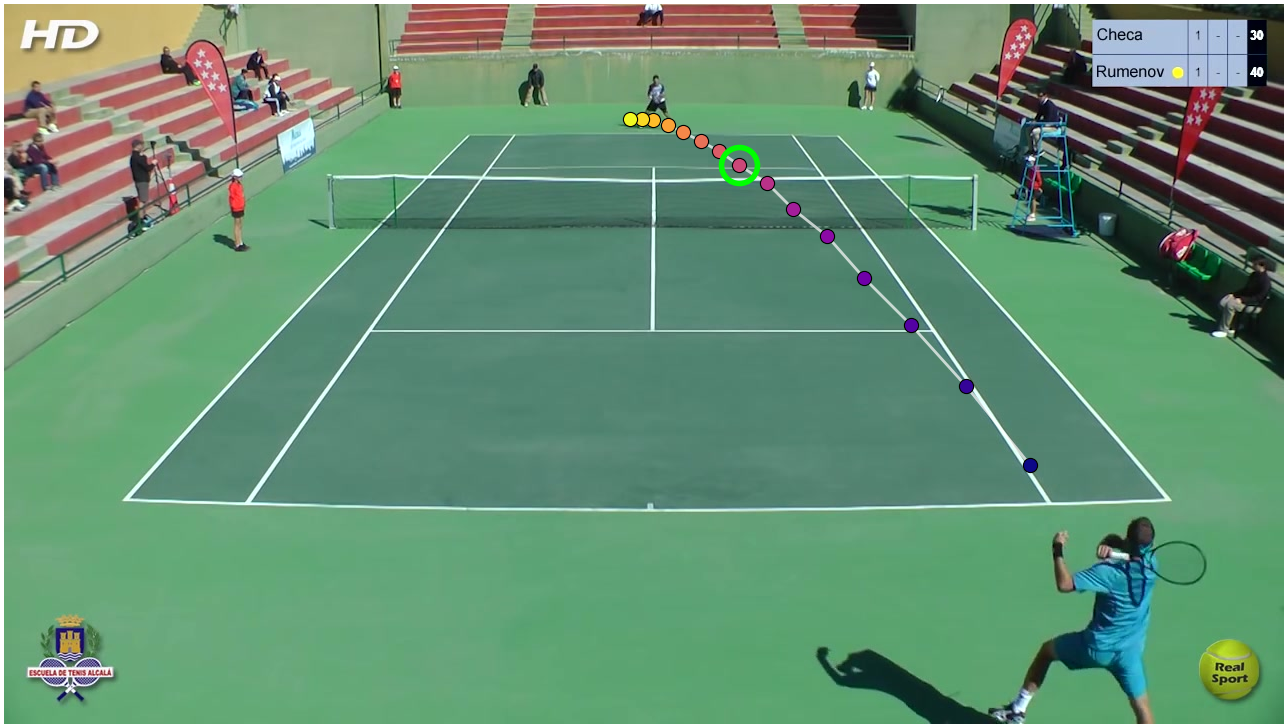
\includegraphics[width=\linewidth]{img/status_class0.png}
    \caption{Status 0: in flight}
  \end{subfigure}\hfill
  \begin{subfigure}{0.32\textwidth}
    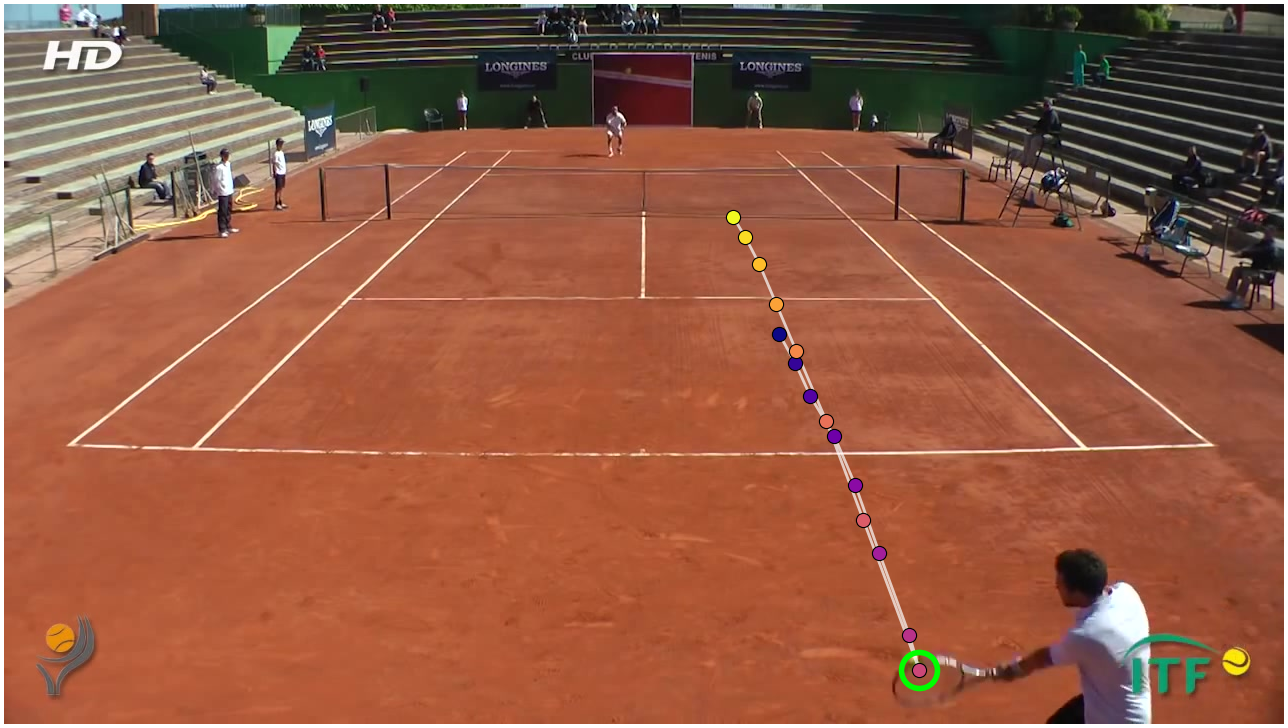
\includegraphics[width=\linewidth]{img/status_class1.png}
    \caption{Status 1: hit}
  \end{subfigure}\hfill
  \begin{subfigure}{0.32\textwidth}
    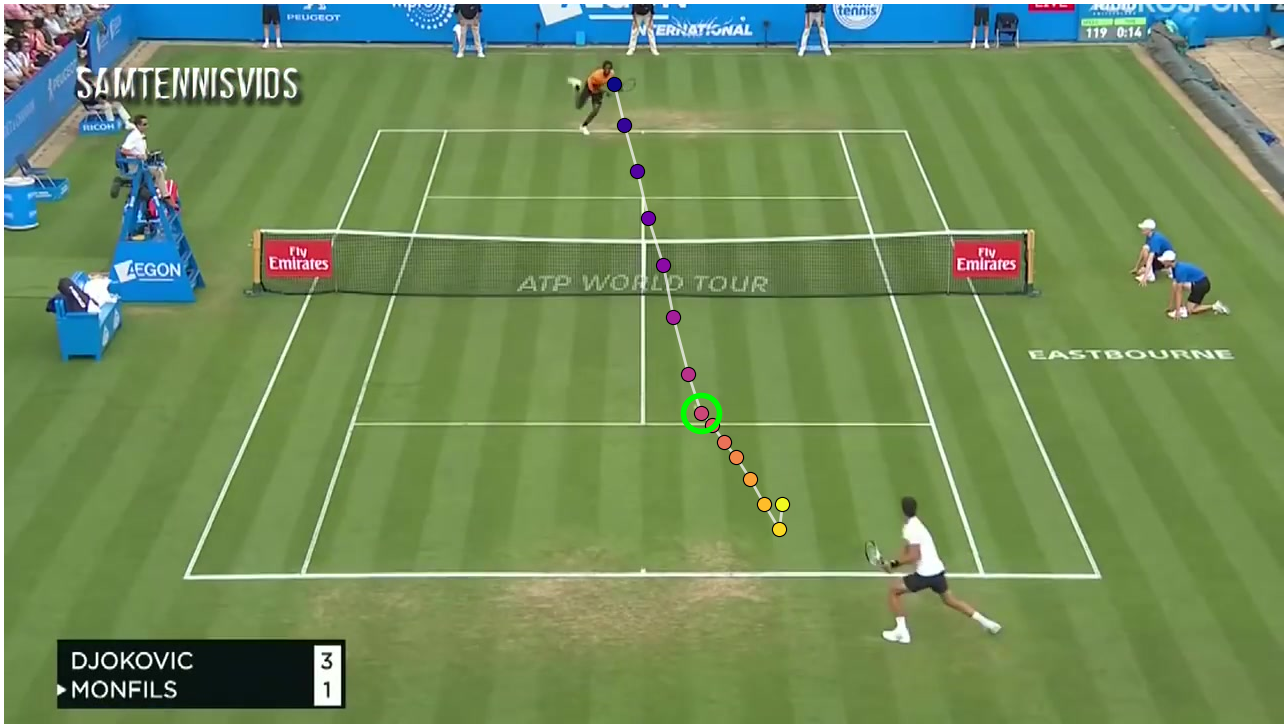
\includegraphics[width=\linewidth]{img/status_class2.png}
    \caption{Status 2: bounce}
  \end{subfigure}
  \caption{The three status values, each shown through the ball trajectory over
    a window of fifteen frames centred on an example event. Points are coloured
    by time (dark to bright), and the green ring marks the labelled frame. An
    in-flight frame lies on a smooth arc, a hit occurs where the ball is struck
    at the player's racket, and a bounce occurs where the ball lands on the
    court. These cues are temporal, which is why bounce detection
    (Chapter~\ref{ch:bounce}) operates on the trajectory rather than on single
    frames.}
  \label{fig:status-classes}
\end{figure}

\section{The Court-Keypoint Dataset}
\label{sec:meth-court}

Court keypoint detection is evaluated on a separate, publicly distributed
dataset, the TennisCourtDetector collection \cite{yastrebksv2023courtdetector},
which is unrelated to the TrackNet tennis data of
Section~\ref{sec:meth-tracknet}. It consists of 8{,}841 single RGB frames at an
original resolution of $1280 \times 720$ pixels, supplied as
``images/\{record\_id\}.png'', together with two JSON annotation files:
``data\_train.json'' with 6{,}630 records and ``data\_val.json'' with
2{,}211 records. Each record provides an identifier and a list of fourteen $[x, y]$ keypoints marking fixed court landmarks
such as the doubles and singles corners, the service points, and the centre
service-line intersections. Figure~\ref{fig:court-gt} shows two annotated frames
with these fourteen keypoints overlaid. The detailed ordering of these fourteen
keypoints, the construction of an inferred court-centre point from the
outer-court diagonals, and the canonical court template used for geometric
registration are specific to the court pipeline and are therefore deferred to
Chapter~\ref{ch:court}; only the dataset's overall size and split, needed to
define the protocol, are stated here.

\begin{figure}[t]
  \centering
  \begin{subfigure}{0.49\textwidth}
    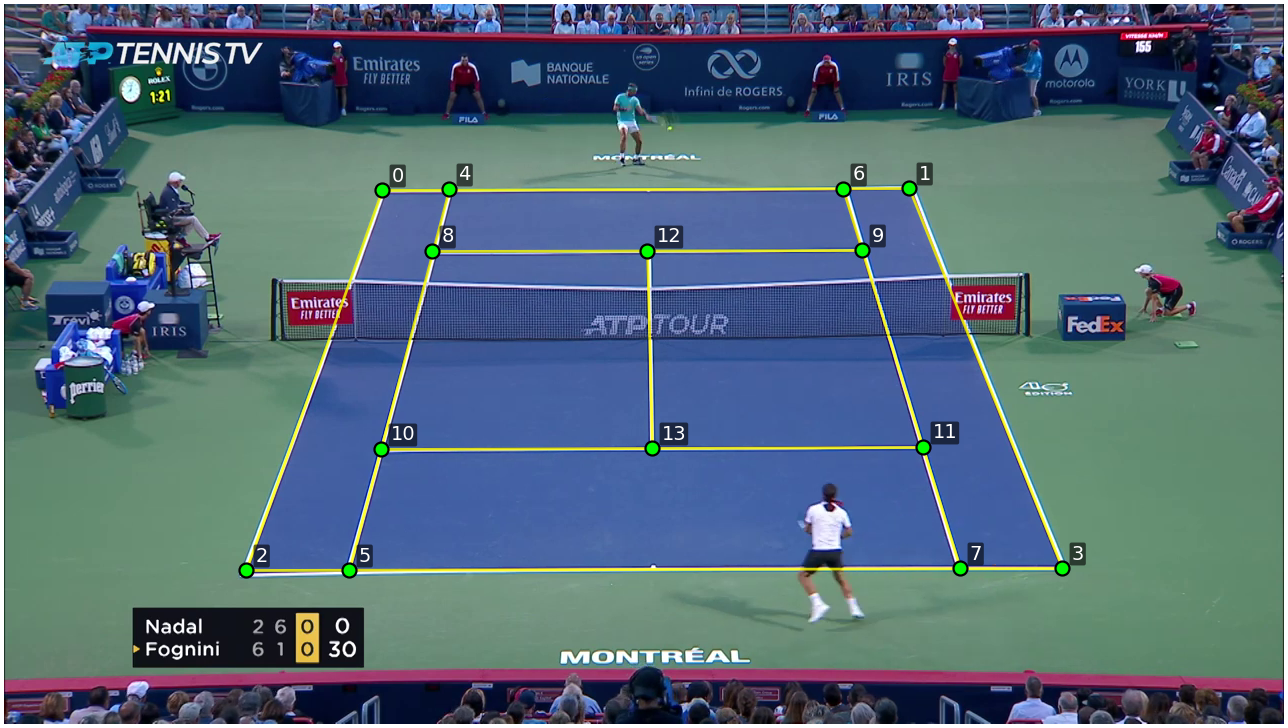
\includegraphics[width=\linewidth]{img/court_gt_example1.png}
    \caption{Hard court}
  \end{subfigure}\hfill
  \begin{subfigure}{0.49\textwidth}
    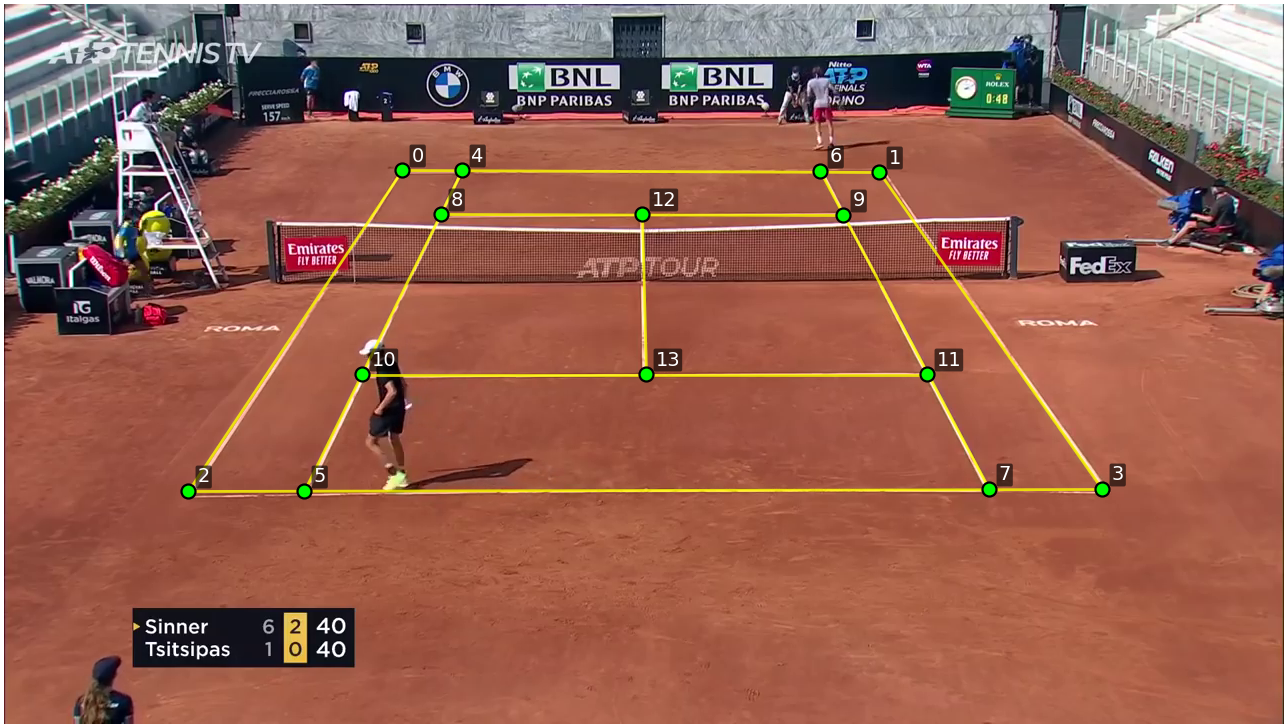
\includegraphics[width=\linewidth]{img/court_gt_example2.png}
    \caption{Clay court}
  \end{subfigure}
  \caption{Two example frames from the court-keypoint dataset with their
    ground-truth annotation overlaid. The fourteen annotated keypoints are shown
    as green markers numbered in the dataset ordering, and the yellow lines are
    the court boundaries they imply. The two frames show different camera angles
    and court surfaces, illustrating the variation the court models must handle.
    The meaning of each keypoint index is given in Chapter~\ref{ch:court}.}
  \label{fig:court-gt}
\end{figure}

\section{Non-Comparability of the Two Datasets}
\label{sec:meth-noncompare}

A point of method that recurs throughout the thesis is stated here once for
clarity. Ball tracking and bounce detection operate on the TrackNet tennis
dataset, whereas court detection operates on the TennisCourtDetector dataset.
The two differ in their content (a small moving ball against broadcast
backgrounds versus static court geometry), in their image resolution and source,
in their annotation schema (per-frame CSV labels versus per-image JSON
keypoints), and in their split policies (Section~\ref{sec:meth-splits}). Because
of these differences, accuracy figures are meaningful only within a
sub-task and must never be compared across sub-tasks. A pixel-accuracy
figure for the ball and a pixel-accuracy figure for court keypoints, for
instance, are measured on different images at different resolutions and do not
constitute a like-for-like comparison. The benchmark of this thesis is therefore
unified within each sub-task rather than across the three.

\section{Split Policies}
\label{sec:meth-splits}

All evaluation in this thesis rests on fixed, deterministic train, validation,
and test splits, so that every model within a sub-task is trained and judged on
exactly the same frames and the results are reproducible from a recorded seed.
The two datasets follow distinct split contracts, which are described in turn
and summarised together in Table~\ref{tab:splits}.

\subsection{TrackNet splits for ball and bounce}
\label{sec:meth-splits-tracknet}

Both TrackNet-based sub-tasks split the data by clip rather than by
frame, so that frames from one clip never appear in more than one split. This is
essential: consecutive frames within a clip are highly correlated, and allowing
them to straddle the train and test boundaries would leak information and inflate
the apparent accuracy. Within this shared principle, however, the two sub-tasks
adopt different partitions of the same 19{,}835-frame pool, reflecting their
different goals.

For ball tracking, matches game1 through game9 are used for
training and validation, and game10 is held out in its entirety as an
unseen test match. Within the training matches, the clips of each match are
shuffled with a fixed seed (42) and partitioned into 85\% training and 15\%
validation. This yields 14{,}812 training frames in 73 clips, 2{,}879
validation frames in 10 clips, and 2{,}144 test frames in 12 clips.

For bounce detection, a separate manifest holds out a different match,
game7, as the test set, because the goal is to measure event timing on a
match whose bounce patterns were never seen in training. The remaining matches
are partitioned into training and validation clips stratified by bounce density,
so that the scarce bounce events are represented in both partitions. This yields
14{,}697 training frames in 71 clips (387 bounce events), 3{,}257 validation
frames in 15 clips (86 bounce events), and 1{,}881 test frames in 9 clips (50
bounce events).

The consequence, made explicit in Table~\ref{tab:splits}, is that even the two
TrackNet sub-tasks draw their test sets from different matches
(game10 for the ball, game7 for bounces) and partition the
remaining data by different rules. Their figures are therefore reported against
different held-out data and are not interchangeable, a finer instance of the
non-comparability principle of Section~\ref{sec:meth-noncompare}.

\subsection{Court split}
\label{sec:meth-splits-court}

The court-keypoint dataset is split deterministically without a random seed.
The 6{,}630 records of ``data\_train.json'' are used as the training set
as supplied. The 2{,}211 records of ``data\_val.json'' are ordered by the MD5 hash of their
record identifier and divided in half: the first 1{,}105
records form the validation set and the remaining records form the test set.
Six test records carrying semantically incorrect annotations are excluded,
leaving 1{,}100 test records.

\begin{table}[h]
  \centering
  \small
  \caption{Split allocations for the three sub-tasks. The two TrackNet sub-tasks
    (ball, bounce) share the same 19{,}835-frame pool but use different held-out
    test matches and different partition rules; the court sub-task uses a
    separate dataset of image records, so its counts are not comparable with the
    TrackNet columns.}
  \label{tab:splits}
  \begin{tabular}{l rr rrr r}
    \toprule
    & \multicolumn{2}{c}{Ball (TrackNet)} & \multicolumn{3}{c}{Bounce (TrackNet)} & Court \\
    \cmidrule(lr){2-3} \cmidrule(lr){4-6} \cmidrule(lr){7-7}
    Split & Frames & Clips & Frames & Clips & Bounces & Records \\
    \midrule
    Train & 14{,}812 & 73 & 14{,}697 & 71 & 387 & 6{,}630 \\
    Val   &  2{,}879 & 10 &  3{,}257 & 15 &  86 & 1{,}105 \\
    Test  &  2{,}144 & 12 &  1{,}881 &  9 &  50 & 1{,}100 \\
    \midrule
    Total & 19{,}835 & 95 & 19{,}835 & 95 & 523 & 8{,}835 \\
    \bottomrule
  \end{tabular}
\end{table}

\section{Shared Evaluation Philosophy and Metric Vocabulary}
\label{sec:meth-metrics}

The comparisons in this thesis are designed so that every model within a
sub-task is scored by an identical, fixed metric suite, computed by shared
evaluation code rather than re-implemented per model. This section defines each
metric once. Which metrics apply to which sub-task is itself task-specific, and
the actual measured values appear in the relevant results chapters. 

\subsection{Localisation metrics}
\label{sec:meth-metrics-loc}

Localisation accuracy, used for both the ball and the court keypoints, is built
on the Euclidean pixel distance between a prediction $\hat{p}_i$ and its
ground-truth position $p_i$,
\begin{equation}
  d_i = \lVert \hat{p}_i - p_i \rVert_2,
  \label{eq:pixdist}
\end{equation}
where both positions are expressed in the original-image pixel space. From this
distance two families of metric are derived.

The first is a thresholded accuracy: the fraction of visible targets whose
prediction falls within a tolerance $\tau$ pixels of the ground truth,
\begin{equation}
  \mathrm{acc@}\tau\mathrm{px} = \frac{1}{|\mathcal{V}|}\sum_{i \in \mathcal{V}}
  \mathbb{1}\!\left[ d_i \le \tau \right],
  \label{eq:accthr}
\end{equation}
where $\mathcal{V}$ is the set of ground-truth-visible targets and
$\mathbb{1}[\cdot]$ is the indicator function. For ball tracking this quantity
is reported at $\tau \in \{5, 10, 20\}$ and written $\mathrm{acc@}\tau$px; for
court keypoints the identical quantity is the percentage of correct keypoints,
written $\mathrm{PCK@}\tau$px, and reported at $\tau \in \{5, 7, 10, 25\}$ with
$\tau = 7$ used as the primary monitoring threshold during training.

The second family reports the mean error directly. The mean absolute error in
pixels, $\mathrm{MAE_{px}}$, is the average of $d_i$ over visible targets. For
ball tracking it is additionally broken down per visibility class (classes 1, 2,
and 3 of Section~\ref{sec:meth-tracknet-schema}; class~0 carries no ball and is
excluded), exposing how localisation degrades as the ball becomes harder to see.
For court keypoints the mean keypoint error is complemented by the median and
maximum keypoint error over detected points, which characterise the typical and
worst-case localisation respectively.

\subsection{Detection metrics}
\label{sec:meth-metrics-det}

Localisation accuracy presupposes that the target was found; detection metrics
measure whether it was found at all. For ball tracking, a binary
visibility decision (does the model report a ball, and is there in fact a ball?)
yields a precision, recall, and $F_1$ from the counts of true positives,
false positives, and false negatives. A stricter, location-aware variant,
following the convention of the TrackNet evaluation \cite{huang2019tracknet},
counts a prediction as a true positive only when the model reports a ball, the
ground truth contains a ball, and the predicted position lies within five pixels
of it; a reported ball that is absent in the ground truth or mislocated beyond
five pixels is a false positive, and a missed visible ball is a false negative.
This produces $\mathrm{precision@5px}$, $\mathrm{recall@5px}$, and
$\mathrm{F1@5px}$, which jointly penalise both missed detections and confident
mislocalisations.
\subsection{Event metrics}
\label{sec:meth-metrics-event}

Bounce detection is scored as an event-timing problem rather than a per-frame
classification problem. Because bounce frames make up under 3\% of the data
(Table~\ref{tab:tracknet-labels}), a per-frame accuracy would be dominated by
the negative class and is deliberately not reported. Instead, each model emits a
per-frame bounce score; this signal is decoded into discrete event
predictions by locating its peaks subject to a minimum spacing between
successive events, and the predicted events are matched to ground-truth
bounces by greedy one-to-one assignment within a temporal tolerance of
$\pm k$ frames. From the resulting true positives, false positives, and false
negatives, an event precision, recall, and $F_1$ at tolerance $k$ are computed
via Equation~\eqref{eq:f1}; the default tolerance is $k = 3$ frames. Two further
summaries characterise behaviour beyond a single operating point: the average
precision (AP), obtained as the area under the precision-recall curve traced by
sweeping the decode threshold, and a tolerance sweep that reports $F_1$ at
$k \in \{0, 1, 2, 3, 5, 7\}$ to show how timing accuracy tightens or relaxes the
score. A bounce-versus-hit confusion count, which buckets each predicted bounce
according to whether the nearest ground-truth event within the tolerance window
is a bounce, a hit, or neither, quantifies the extent to which racket hits are
mistaken for bounces. It should be noted that AP and $F_1$ at a tolerance are
different quantities at different operating points and are not interchangeable; a
comparison between them is made only at a fixed tolerance, never as a single
headline gap.

\subsection{Geometric and efficiency metrics}
\label{sec:meth-metrics-geom}

For the court sub-task, keypoint accuracy is supplemented by metrics that
measure the quality of the downstream geometric registration. A homography is
estimated from the predicted keypoints, the visible ground-truth keypoints are
projected through it into the canonical court plane, and their displacement from
the template is reported in centimetres as a mean and a maximum reprojection
error, alongside the rate at which a homography could be estimated at all. The
estimation procedure itself, including its robust fitting and the canonical
court template, is described where it is used, in Chapter~\ref{ch:court}.

Finally, efficiency is reported uniformly across all sub-tasks through two
quantities: the inference throughput in frames per second (FPS), and the model
size as a parameter count in millions. These allow the accuracy of each model to
be read against its computational cost, which is key idea to the accuracy-versus-
speed trade-offs examined in the results chapters and to the model-selection
rationale of the integrated system (Chapter~\ref{ch:integrated}).

With the datasets, split contracts, and metric definitions now fixed, the
following three chapters apply this protocol in turn: ball tracking in
Chapter~\ref{ch:ball}, court keypoint detection and homography in
Chapter~\ref{ch:court}, and bounce-event detection in Chapter~\ref{ch:bounce}.
Each of those chapters also describes the training details specific to its
models, including the optimiser, loss function, and hyperparameters.
